\section{Introduction} % (fold)
\label{sec:Introduction}

\subsection{Problématique et contexte} % (fold)
\label{sub:prob_contexte}

Le club étudiant Chinook\footnote{\url{http://chinookets.com}} de l'ÉTS est un regroupement d'étudiants qui analysent, concoivent et construisent un véhicule propulsé par une éolienne [figure \ref{fig:chinookHall}]. Le véhicule participe, chaque année, depuis deux années à une compétition de véhicules du même type et participe à des courses contre la montre. Le véhicule est ensuite évalué selon sa performance en fonction de sa vitesse par rapport à la vitesse du vent.

La compétition vise à ammener les étudiants a développer de nouvelles technologies pour les éoliennes, plus précisément pour des éoliennes de petites dimensions. Afin de rendre la compétition intéressante, elle sont utilisées en tant que moteur d'un véhicule de petite dimension. Un tel véhicule ne serait pas viable mais une telle technologie pourrait facilement être adapté sur d'autre médiums tels que les éoliennes sur des navires ou pour des batiments.

\begin{figure}[H]
  \centering
  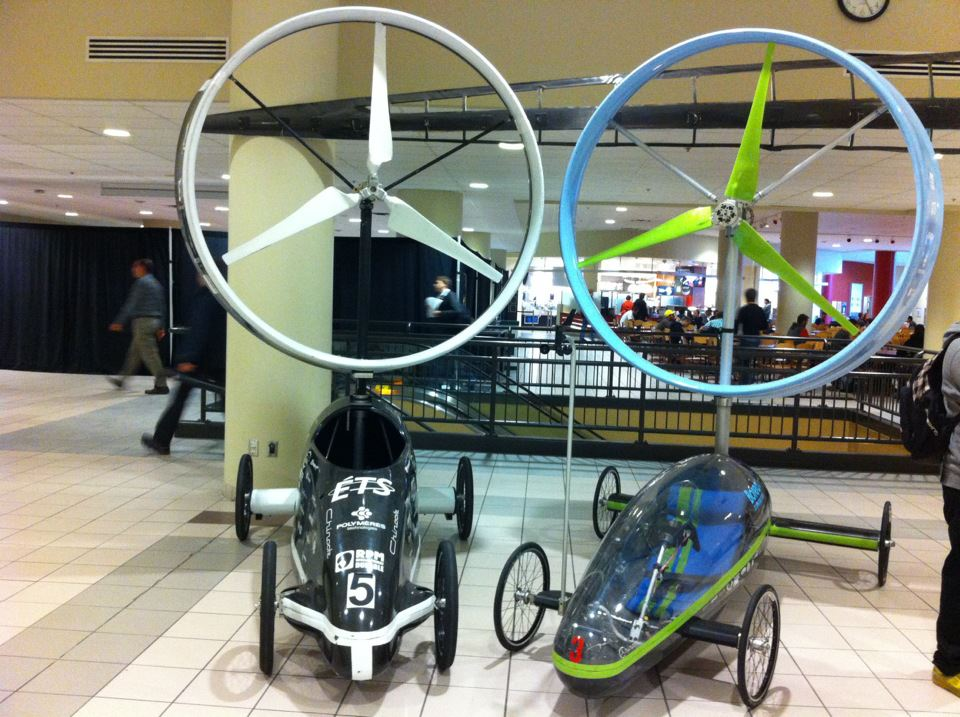
\includegraphics[width=0.5\textwidth]{images/chinook_1_2.jpg}
  \caption[Chinook 1 et 2]{Le Chinook 1 et le Chinook 2 en exposition dans le Hall A de l'ÉTS}
  \label{fig:chinookHall}
\end{figure}

Pour améliorer le véhicule, permettre de à l'équipe de bien performer et rester compétitif l'équipe installe un système électro-mécanique de contrôle de l'angle d'attaque des pâles. La transmission du véhicule sera aussi modifiée afin de pouvoir être asservi électroniquement.

Afin de pouvoir contrôller ces systèmes électroniques, des modèles de contrôle et d'optimisation de la puissance de l'éolienne doivent être créés. Les modèles disponibles sur les éoliennes statique peuvent s'appliquer pour une éolienne en mouvement mais doivent être modifiés afin de prendre en compte plusieurs facteurs.

\citet{LaksPao} décris plusieurs méthodes de contrôle des éoliennes mais la plupart de ces méthodes ne vont pas chercher le point maximum de puissance, elle vont plutôt chercher un point stable de contrôle qui permet d'offrir une puissance stable pour les générateurs électrique. \citet{Jelavic05} va chercher le point maximum de puissance de l'éolienne, mais seulement dans le cas oùla vitesse du vent est sous la vitesse prescrite de l'éolienne. \citet{Ouissam12} dans son article utilise un algorithme génétique couplé a un algorithme flou (fuzzy control system), la méthode semble fonctionner mais celui-ci ne semble pas prendre en compte les changements de vitesse de rotation de l'éolienne et les variations de la vitesse du vent.

% subsection Problématique et contexte (end)
\subsection{Objectifs} % (fold)
\label{sub:Objectifs}


Le présent projet à pour but d'ammener l'éolienne du Chinook 3 [figure: \ref{fig:matRotor}] à opérer dans les conditions et à l'aide des paramètres d'opérations les plus optimales possibles. Pour ce faire, l'éolienne doit être caractérisé, un modèle de contrôle et d'optimisation de l'angle d'attaque ($\beta$) des pales et du ratio de transmission qui affecte la vitesse de rotation de l'éolienne ($\omega$) doit être conçu, analysé puis ce modèle doit être implanté dans le logiciel de la carte électronique de calcul.

Le système de contrôle pourra, à tout moment et selon certaines conditions, changer l'angle d'attaque des pales ($\beta$) où le ratio transmission afin d'atteindre les performances optimales de l'éolienne dans les conditions de vitesse du véhicule et de vitesse du vent.

\begin{figure}[H]
  \centering
  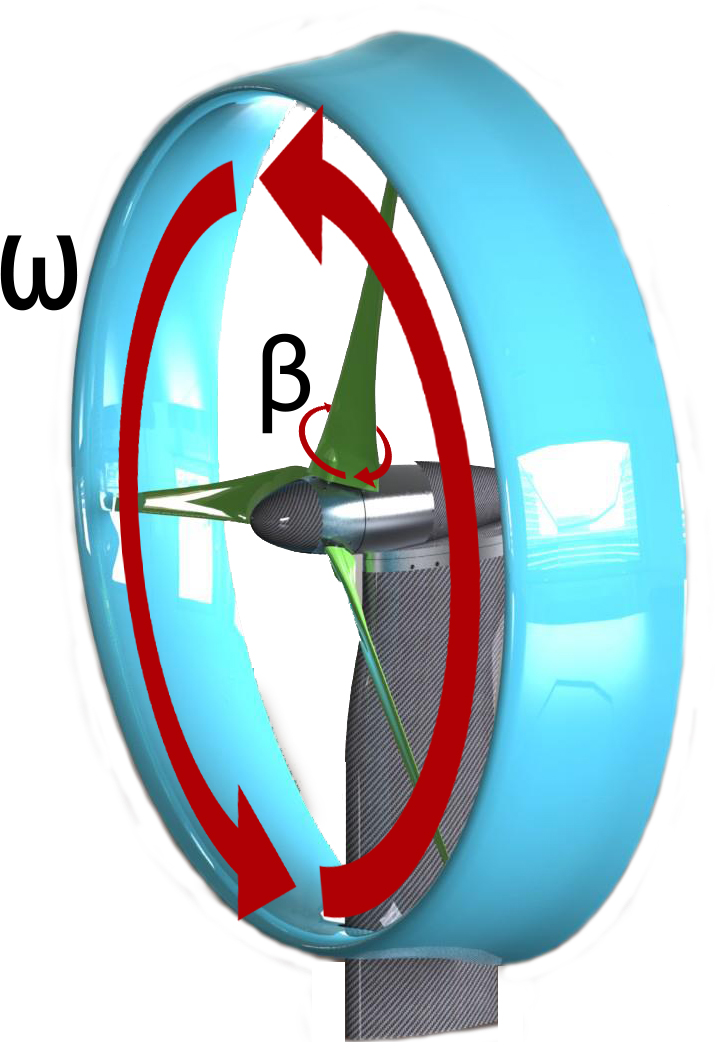
\includegraphics[width=0.5\textwidth]{images/mat_rotor_annote.jpg}
  \caption[Mat et Rotor du Chinook 3]{Rendu 3D du mat et du rotor du Chinook 3}
  \label{fig:matRotor}
\end{figure}

Un tel modèle ainsi opérationnel dans les systèmes de contrôle du Chinook permettra au véhicule d'atteindre de meilleures vitesses et ce plus rapidement tout en permettant de conserver les vitesses atteintes et de mieux résister aux turbulences environnementales que par les années passées.

% subsection Objectifs du projet (end)

% section Introduction (end)
